\documentclass[11pt,openany]{book}
\usepackage{blindtext}
\usepackage{tikz,tcolorbox}
\usepackage{xcolor}
\usepackage{amsfonts}
\usepackage{hyperref} 
\usepackage{indentfirst}
\usepackage{graphicx}
\usepackage[normalem]{ulem}
\usepackage [english]{babel}
\usepackage [autostyle, english = american]{csquotes}
\usepackage{appendix}
\usepackage{tabularx}
\usepackage{amsmath,amssymb}
\usepackage{mathtools}
\usepackage{makecell}
\graphicspath{ {./images/} }
\usepackage{enumitem}
\usepackage{soul}
\usepackage{mathtools}
\usepackage{wrapfig}
\usepackage{mathrsfs}
\usepackage{centernot}
\usepackage{amsthm}
\usepackage{listings}
\usepackage{biblatex}
\addbibresource{bibliograph.bib}

\usepackage{pagenote}


\definecolor{codegreen}{rgb}{0,0.6,0}
\definecolor{codegray}{rgb}{0.5,0.5,0.5}
\definecolor{codepurple}{rgb}{0.58,0,0.82}
\definecolor{backcolour}{rgb}{0.95,0.95,0.92}

\lstdefinestyle{mystyle}{
	backgroundcolor=\color{backcolour},   
	commentstyle=\color{codegreen},
	keywordstyle=\color{magenta},
	numberstyle=\tiny\color{codegray},
	stringstyle=\color{codepurple},
	basicstyle=\ttfamily\footnotesize,
	breakatwhitespace=false,         
	breaklines=true,                 
	captionpos=b,                    
	keepspaces=true,                 
	numbers=left,                    
	numbersep=5pt,                  
	showspaces=false,                
	showstringspaces=false,
	showtabs=false,                  
	tabsize=2
}

\lstset{style=mystyle}
%% End notes to be printed as sections at the
%% end of each chapter.
\renewcommand*{\notedivision}{\section*{\notesname}}
\renewcommand*{\pagenotesubhead}[1]{}

\newcommand*{\exercises}{\section*{\exercisename}}
%%%%%%%%%%%%% For customising the endnote markers. Comment these out if you don't want them.
% To prefix each note number with the chapter number
\renewcommand{\thepagenote}{\thechapter-\arabic{pagenote}}

% To have a slightly different formatting for the endnote numbers in the text -- smaller text, sans-serif, square brackets
\renewcommand\notenumintext[1]{\space{\footnotesize\sffamily[FN-#1]}}

% To have a slightly different formatting for the endnote numbers in the notes section. Just the square brackets and sans-serif; normal size.
\renewcommand\notenuminnotes[1]{{\sffamily[FN-#1] }}

% If you want a different name/heading for the end notes
\renewcommand{\notesname}{End Notes}
\newcommand{\exercisename}{Exercises}
%%%%%%%%%%%%% End customisation

\newcommand{\definition}[2]{\begin{tcolorbox}[title=Definition ({#1}),colframe=black]{#2}\end{tcolorbox}
}
\newcommand{\proposition}[1]{\begin{tcolorbox}[title=Proposition,colframe=red!50!blue!20!white,colback=red!35!blue!10!white, coltitle=black]{#1}\end{tcolorbox}
}
\newcommand{\theorem}[2]{\begin{tcolorbox}[title=Theorem ({#1}),colframe=red!70!black,colback=red!5!white]{#2}\end{tcolorbox}
}
\newcommand{\example}[1]{\begin{tcolorbox}[title=Example,colframe=yellow!50!white,colback=yellow!20!white,coltitle=black]{#1}\end{tcolorbox}
}
\newcommand{\corollary}[1]{\begin{tcolorbox}[]{Corollary: {#1}}\end{tcolorbox}
}
%\newcommand{\exercises}{\section*{\exercisename}}
%% THIS LINE IS MANDATORY
\makepagenote

\begin{document}
	
	\chapter{Sample: vector calculus}
	
	%in the actual thing, would ideally create a macro to have piecewise smooth reference the definition (in pdf
	[input definitions of parametrization and orientation]
	\definition{Line Integral: scalar}{
		Let $U \subset \mathbb{R}^n$, $\gamma \subset U$ be a smooth oriented curve, and $f: U \to \mathbb{R}$. The \textbf{line integral of $f$ along $\gamma$} is defined as
		\[
		\int_\gamma \ f \ ds \ = \ \int_a^b f(r(t)) \ |r'(t)| \ dt
		\]
		where $r : [a,b] \to \gamma$ is any parameterization of $\gamma$.

		If $\gamma =  \gamma_1 \cdot \gamma_2 \cdot ... \cdot \gamma_n  $ is piecewise smooth, where $\gamma_j$ is smooth,

		\[
		\int_\gamma \ f \ ds \ = \int_{\gamma_1} \ f \ ds + ... + \int_{\gamma_n} \ f \ ds
		\]
	}
	\definition{Line Integral: vector}{
		Let $U \subset \mathbb{R}^n$, $\gamma \subset U$ be a smooth oriented curve, and $f: U \to \mathbb{R}^n$. The \textbf{line integral of $f$ along $\gamma$} is defined as
		\[
		\int_\gamma \ f  \cdot ds \ = \ \int_a^b f(r(t)) \cdot r'(t)  \ dt
		\]
		where $r : [a,b] \to \gamma$ is any parameterization of $\gamma$.

		If $\gamma =  \gamma_1 \cdot \gamma_2 \cdot ... \cdot \gamma_n  $ is piecewise smooth, where $\gamma_j$ is smooth,
		\[
		\int_\gamma \ f \cdot ds \ = \int_{\gamma_1} \ f \cdot ds + ... + \int_{\gamma_n} \ f \cdot ds
		\]
	}

	The line integral does not depend on the parameterization of $\gamma$. One exercise will guide you through the proof.
	\section*{Geometric intuition}
	%todo - plot in python
	\example{
		Let $\gamma$ be the segment of the curve $y=x^3$ for $-1\leq x\leq 1$ starting at $(-1,-1)$.
		Express 
		\[
		\int_{\gamma} (x^2 +y^2) ds
		\]
		as a single variable integral.
	}
	For a visualization, let's plot a 2D function (so visualizing the graph in 3D) in Python. $\gamma$ can be parametrized as $r(t) = (t,t^3)$ for $t\in[-1,1]$.
	\begin{lstlisting}[language=Python]
import matplotlib.pyplot as plt
import numpy as np
#create figure
fig=plt.figure(figsize=(5,4))
ax = fig.add_subplot(projection='3d')

#plot sin(x+y)
X,Y=np.meshgrid(np.linspace(-1,1,10), np.linspace(-1,1,10))
Z=(X**2)+Y**2
surface=ax.plot_surface(X, Y, Z, alpha=0.5,
label='graph surface')
ax.set_xlabel('x')
ax.set_ylabel('y')
ax.set_zlabel('x^2 + y^2')

#plot the curve and the cross section to integrate
curve=np.linspace(-1,1,50)
plot_curve=ax.plot(curve, curve**3, 0,
label='cross section to integrate',color='red')
curvevalues=curve**2 + curve**2**3
curveonsurface=ax.bar3d(curve, curve**3,0,
dx=0.01, dy=0.01, dz=curvevalues, alpha=0.5,
color='red')

#show curve
plt.legend()
plt.show()
	\end{lstlisting}

	\begin{wrapfigure}{r}{0.6\textwidth} 
		\centering
		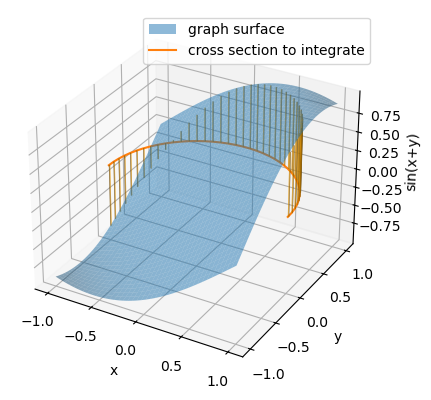
\includegraphics[width=0.6\textwidth]{sin.png}
	\end{wrapfigure}
	This scalar line integral represents the signed cross-section area of the graph along the curve, and is colored in orange on the left figure.
	What we need to do now is to unroll this cross section into 2D and perform a Riemann integral. However, a simple 
	\[
		\int_{-1}^{1} \ t^2 + (t^3)^2 \ dt
	\]
	does not work - some parts of the curve are stretched and others are compressed. The red vertical bars are evenly spaced in t, but are denser near the origin. How much is this stretch/compression factor? 
	It is represented by how quickly the curve is moving with respect to t, which is exactly $|r'(t)|$.
	Since $r'(t) = \begin{pmatrix}
		1 \\ 3t^2
	\end{pmatrix}$, the full computation is
	\begin{align*}
		\int_\gamma x^2+y^2 ds &= \int_{-1}^1 (t^2+t^6)  \ \left|\begin{pmatrix}
			1 \\ 3t^2
		\end{pmatrix}\right| \ dt \\
		&= \int_{-1}^{1} (t^2+t^6) \sqrt{1+9t^4} \ dt
		\\
	\end{align*}

	\example{
		Let $\gamma$ be the segment of the curve $y=x^3$ for $0<x<1$ starting at $(0,0)$.
		Compute 
		\[
		\int_{\gamma} \begin{pmatrix}
			x^2 \\ y^2
		\end{pmatrix} \cdot ds
		\]
		.
	}
	For vector line integrals, we integrate the \textbf{projection} of $f$ onto the curve, so we can think of it as a scalar integral \[
		\int_a^b \left[ f(r(t)) \cdot \frac{r'(t)}{|r'(t)|}  \right]   |r'(t)| \ dt
	\]
	. The first term is the signed length of the projection of $f$ onto the tangent vector, the scalar we want to integrate.
	\\
	We can parametrize $\gamma$ as $r(t) = (t,t^3)$ as $t$ goes from $0$ to $1$.
	The explicit formula is \begin{align*}
		\int_{\gamma} \begin{pmatrix}
			x^2 \\ y^2
		\end{pmatrix} \cdot ds &= \int_{0}^1 \begin{pmatrix}
			t^2 \\ t^6
		\end{pmatrix} \cdot  \begin{pmatrix}
			1 \\ 3t^2
		\end{pmatrix} \ dt
		\\
		&= \int_0^1 t^2+3t^8 dt \\
		&= \frac{2}{3}.
	\end{align*}
	\example{
		Previous example rephrased in physics terms:\\
		Alice is pushing a box. After $t$ seconds, the box is at $(t,t^3)$. Alice's force on the box at $(x,y)$ can be modelled by
		$x^2 \ \hat{i} + y^2\ \hat{j}$. After $1$ second, how much work did Alice do on the box?
	}
	You might also recognize vector line integrals from the formula for work \[
	W = \int \vec{F} \cdot d\vec{s} 
	\]
	in first quarter physics. If we parametrize $\gamma$ as ${r}(x)$ for $x \in [0,t]$, we get 
	\begin{align*}
		W &= \int_0^t \ \vec{F}(r(t)) \cdot {r}'(t) dt \\
		&= \int_0^t \vec{F} \cdot v(t) dt \textrm{, $v$ denotes velocity}
	\end{align*}
	This is the same as ``work equals to the integral of power with respect to time"!
	
	\exercises
	computation exercises follow...
	\begin{enumerate}
		\item The length of a curve can be obtained by integrating a constant with respect to ds. What is this constant that makes the cross section area equal (in value) to the arc length? 
		\item compute the length of the following curves : aaa, bbb, ccc
		\item compute the following line integrals : ddd, eee, fff
	\end{enumerate}
	
	\section*{Fundamental Theorem of Line Integrals}
	We want to build toward something that looks like 
	\[
		\int_{a}^{b} f(x) \ dx = F(b) - F(a)
	\], something similar in line integrals would be \[
		\int_\gamma f \cdot ds = F(b) - F(a)
	\] where $a$ and $b$ are the end points of $\gamma$. This is unfortunately not true from [one of the previous exercises]. So what can we do? We define this to be a property of a special set of vector-valued functions, and see what other properties this gives us.
	
	
	\proposition{
		Let $U\subset\mathbb{R}^n$ be open, $f:U\to\mathbb{R}^n$ be continuous, and $F:U\to\mathbb{R}$ satisfy the condition that for every piecewise smooth oriented curve $\gamma$ parametrized by $r: [a,b]\to U$
		\[
		\int_\gamma f \cdot ds = F(r(b)) - F(r(a)).
		\] 
		Then, \[
			f = \nabla F.
		\]
	}
	\begin{proof} \ \\
		Idea: we consider the partial derivatives of $F$. Without loss of generality, it is enough to consider the partial derivative in the first variable $x$. \\
		Let $\vec{p} \in U$, we want to show that $\frac{\partial F}{\partial x} \big| _{\vec{p}} = f(\vec{p}) \cdot \vec{e}_1$. We can also consider the straight line $\gamma_h(t) = \vec{p} + t\vec{e}_1$ for $t\in[0,h]$. We then have \begin{align*}
			\frac{\partial F}{\partial x} \big| _{\vec{p}} &= \lim_{h\to 0} \frac{F(\vec{p}+h\vec{e}_1)-F(\vec{p})}{h} \\
			&= \lim_{h\to 0} \frac{\int_{\gamma_h} f \cdot ds}{h}\\
			&= \lim_{h\to 0} \frac{\int_0^h f(\vec{p}+t\vec{e}_1) \cdot \vec{e}_1 \ dt}{h}
		\end{align*}
		The last expression is the (one dimensional) derivative of the function $g(x)=\int_0^x f(\vec{p}+t\vec{e}_1) \cdot \vec{e}_1 \ dt$ at $x=0$, so equals $f(\vec{p})\cdot \vec{e}_1$ from the Fundamental Theorem of Calculus.
	\end{proof}
	
	We thus motivate the following definition:
	\definition{Conservative Vector Fields}{
		Let $U\subset\mathbb{R}^n$ be open, $f:U\to\mathbb{R}^n$ be continuous. We say that $f$ is \textbf{conservative} if
		$f = \nabla F $ for some scalar valued function $F:U\to\mathbb{R}$.
		If such an $F$ exists, we call it a \textbf{scalar potential} of $f$.
	}
 
	
	As a bonus, we get the uniqueness of $F$.
	\proposition{
		If such an $F$ exists, it is unique up to addition of a constant on each connected subset of $U$.
	}
	
	\begin{proof}
		Let $f=\nabla G$. Then $\nabla(F-G)=\nabla F - \nabla G = f-f =0$, so that $F-G$ is constant on each connected subset.
	\end{proof}
	Informally, $F$ is some sort of ``antiderivative" of $f$.
	\theorem{Gradient}{
		Let $U\in\mathbb{R}^n$ be open, $F:\mathbb{R}^n\to\mathbb{R} \ C^1$, $\gamma\in U$ be a piecewise smooth oriented curve starting at $\vec{a}$ and ending at $\vec{b}$
		then \[
		\int_\gamma \nabla F \cdot ds = F(\vec{b})-F(\vec{a})
		\]
	}
	\begin{proof}
		Consider the case where $\gamma$ is smooth and parametrized by $r:[a,b]\to U$. Then
		\begin{align*}
			\int_\gamma \nabla F \cdot ds &= \int_a^b \nabla F(r(t)) \cdot r'(t) dt \\
			&= \int_a^b \frac{d F(r(t))}{dt} \ dt \textrm{ (chain rule)}\\
			&= F(r(\vec{b})) - F(r(\vec{a})) \textrm{ (Fundamental Theorem of Calculus)}
		\end{align*} 
		The case where $\gamma$ is piecewise smooth is similar, you should get a telescoping series by applying the Gradient Theorem to each smooth piece of $\gamma$.
	\end{proof}
	\example{
		A particle starts from $(0,0,0)$ and does the following:
		\begin{enumerate}
			\item move $1/10$ units in $x$
			\item move $1/10$ units in $y$
			\item move $1/10$ units in $z$
			\item repeat first three moves until it reaches $(1,1,1)$
		\end{enumerate}
		Compute the line integral of $f(x,y,z)= (yz,xz,xy)$ along the path $\gamma$ traced by the particle.
	}
	... what? $\gamma$ is intentionally complicated here, but you can definitely compute the integral as a summation of $30$ line integrals.
	As a visualization exercise, try to predict what $\gamma$ looks like.
	
	\begin{lstlisting}[language=Python]
		import matplotlib.pyplot as plt
		import numpy as np
		#create figure
		fig=plt.figure(figsize=(5,4))
		ax = fig.add_subplot(projection='3d')
		N=10
		p_j=[i/N for i in range(N)]
		X=[j for i in p_j for j in [i,i+1/N,i+1/N] ]+[1]
		Y=[j for i in p_j for j in [i,i,i+1/N] ]+[1]
		Z=[j for i in p_j for j in [i,i,i] ]+[1]
		plt.plot(X,Y,Z)
		plt.show()
	\end{lstlisting}
	
	Before we do any annoying computation... could this be a conservative vector field? We want scalar function that is $yz$ differentiated with respect to (wrt) $x$, $xz$ differentiated wrt $y$, $xy$ differentiated wrt $z$.
	\begin{wrapfigure}{r}{0.6\textwidth}
		\centering
		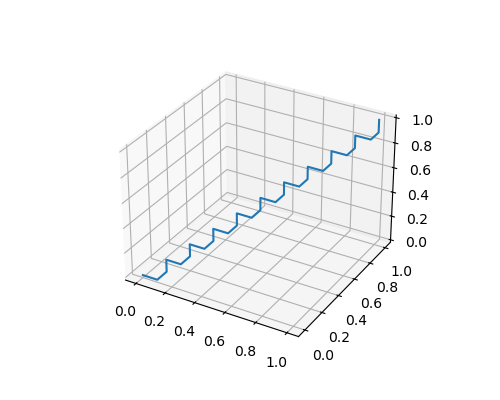
\includegraphics[width=0.6\textwidth]{staircase.png}
	\end{wrapfigure}
	One solution is $F(x,y,z)=xyz$, which you can check very quickly it gives the correct partial derivatives.
	Now we apply the Fundamental Theorem of Line Integrals to show that
	\[
	\int_{\gamma} f\cdot ds = F(1,1,1) - F(0,0,0) = 1
	\]\
	 Much shorter!
	For this problem, $\gamma$ looks like a staircase, but we could replace it with any curve that starts at $(0,0,0)$ and ends at $(1,1,1)$. The answer will still be the same.
	\subsection{Path Independence}
	\definition{Path Independent Vector Fields}{
		Let $U\subset\mathbb{R}^n$ be open, $f:U\to\mathbb{R}^n$ be continuous. We say that $f$ is \textbf{path-independent} if for every pair of curves
		$\gamma_1$ and $\gamma_2$ with the same starting points and ending points, \[
		\int_{\gamma_1} f \cdot ds = \int_{\gamma_2} f \cdot ds
	\].
	}
	\proposition{
		$f$ is path-independent if and only if $\int_\gamma f\cdot ds =0$ for every piecewise-smooth closed curve $\gamma$.
	}
	\begin{proof}
		[placeholder]
	\end{proof}
	A quick corollary of the Gradient Theorem is that gradients are path-independent.
	\corollary{
	Let $f$ be conservative, and $\gamma_1$ and $\gamma_2$ be two curves with the same starting points and ending points. Then \[
		\int_{\gamma_1} f \cdot ds = \int_{\gamma_2} f \cdot ds
	\].
	}
	
	\begin{proof}
		Here is a hint:
		Let $\gamma_1$ and $\gamma_2$ start at $\vec{a}$ and end at $\vec{b}$, then apply the Gradient Theorem.
	\end{proof}
	Under some conditions,These few properties are actually equivalent to the definition of conservative vector fields!
	\theorem{Gradient (converse)}{
		Let $U\in\mathbb{R}^n$ be open and \textbf{connected}, $f:U\to\mathbb{R}^n$. \\
		Then $f$ is conservative if and only if $f$ is path-independent.
	}
	\begin{proof}
		$\implies$ is the Gradient Theorem.\\
		$\impliedby$:
		We define $F$ by a line integral.
		Let $x \in U$, and $F(y) = \int_\gamma f \cdot ds$, where $\gamma$ is a (piecewise) smooth from $x$ to $y$.
		Because the integral is same regardless of the path, $F$ is well-defined.
		So that for every curve $\Gamma$that goes from $a$ to $b$, replace the line integral with a path $\gamma_1$ that goes from $a$ to $x$
		and $\gamma_2$ that goes from $x$ to $b$.
		so that \begin{align*}
			\int_\Gamma f\cdot ds &= \int_{\gamma_1} f\cdot ds + \int_{\gamma_2} f\cdot ds \\
			&= - (F(a) - F(x) ) + (F(x) + F(b))\\
			&= F(b) - F(a)
		\end{align*}
		By a proposition we have proved earlier, $f=\nabla F$ and is conservative. 
	\end{proof}
	
	\exercises
	\begin{enumerate}
		
		\item For this question, take for granted that the derivative of $\tan^{-1}(x) = 1/(1+x^2)$. \begin{enumerate}
			\item Verify that $\nabla \tan^{-1}(y/x) = (\frac{-y}{x^2+y^2}, \frac{x}{x^2+y^2})$.
			\item Integrate $(\frac{-y}{x^2+y^2}, \frac{x}{x^2+y^2})$ over the unit circle, oriented counter-clockwise.
			\item Is $\nabla \tan^{-1}(y/x)$ conservative? When can you apply the Gradient Theorem to this function? Some interesting phenomena arise from this ``paradox", as an example, see the Aharonov-Bohn Effect.
		\end{enumerate}
		\item Let $f:\mathbb{R}^n\setminus\{\vec{0}\} \to\mathbb{R}^n$ be continuous and radially symmetric. That is, there is some scalar function $k$ such that $f(\vec{x})= k(|\vec{x}|) \ \vec{x}/ |\vec{x}|$. [ideally want to plot something here] \begin{enumerate}
			\item What is the line integral of $f$ along any circlular arc $C$ centered at the origin? Conclude that if $f$ is conservative, its scalar potential has to be radially symmetric too. 
			That is, the value of $F(\vec{x})$ is only dependent on $|\vec{x}|$.
			\item Integrate $f$ over a (well-chosen) path to find a scalar potential for $f$.
			\item Justify the terminology for gravitational, elastic, and electric \textbf{potential}.  
		\end{enumerate}
		
	\end{enumerate}
	
\end{document}